\hypertarget{relations_8cpp}{}\section{O\+L13/relations.cpp File Reference}
\label{relations_8cpp}\index{O\+L13/relations.\+cpp@{O\+L13/relations.\+cpp}}


Définitions des fonctions déclarées dans le \hyperlink{relations_8h_source}{relations.\+h}.  


{\ttfamily \#include \char`\"{}relations.\+h\char`\"{}}\newline
{\ttfamily \#include \char`\"{}sstream\char`\"{}}\newline
Include dependency graph for relations.\+cpp\+:\nopagebreak
\begin{figure}[H]
\begin{center}
\leavevmode
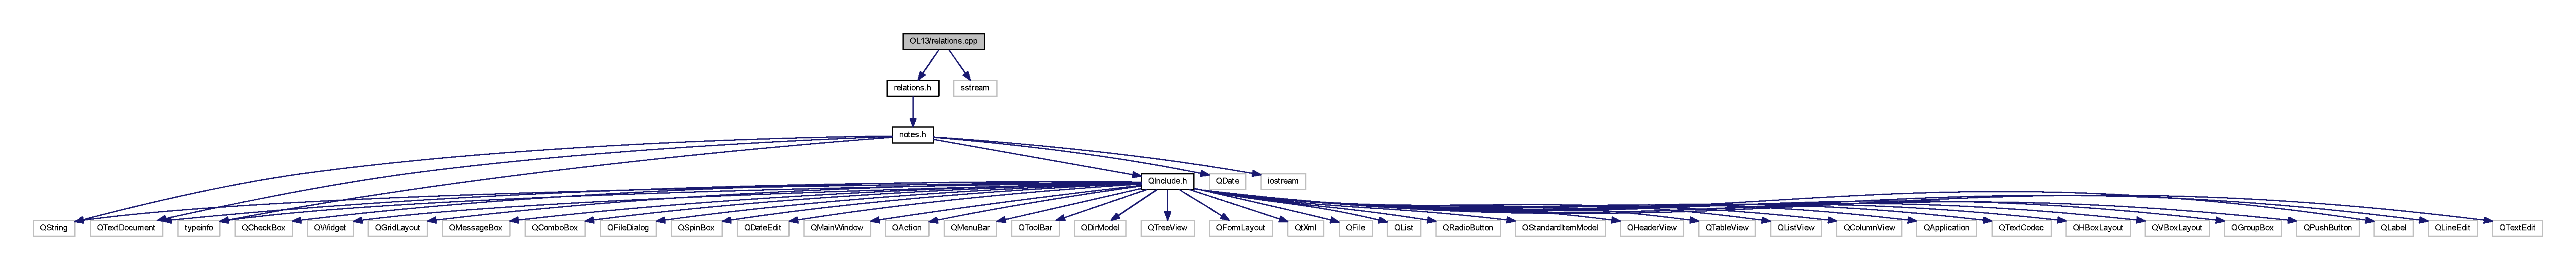
\includegraphics[width=350pt]{relations_8cpp__incl}
\end{center}
\end{figure}


\subsection{Detailed Description}
Définitions des fonctions déclarées dans le \hyperlink{relations_8h_source}{relations.\+h}. 

\begin{DoxyAuthor}{Author}
Garnier Maxime, Naudin Louise, Pépin Hugues 
\end{DoxyAuthor}
\begin{DoxyVersion}{Version}
1.\+0 
\end{DoxyVersion}
\begin{DoxyDate}{Date}
14 Juin 2017
\end{DoxyDate}
Classes présentes \+:
\begin{DoxyItemize}
\item \hyperlink{class_notes_couple}{Notes\+Couple} La classe \hyperlink{class_notes_couple}{Notes\+Couple} est en agrégation avec la classe \hyperlink{class_relation}{Relation} \+: une relation contient un ensemble de couple de notes. Dans le cas où l\textquotesingle{}ensemble des couples d\textquotesingle{}une relation est supprimé, la relation existe toujours mais est vide. Elle pourra être repeuplée par de nouveaux couples.

La classe \hyperlink{class_notes_couple}{Notes\+Couple} possède deux attributs noteX et noteY pointant chacun sur une note du couple, un attribut pour le label du couple et un attribut booléen spécifiant si le couple est symétrique. C\textquotesingle{}est à dire que la relation va de noteX vers noteY et réciproquement.

La classe \hyperlink{class_notes_couple}{Notes\+Couple} est composée par la classe Notes \+: si les notes sont supprimées, les couplent n\textquotesingle{}existent plus non plus.
\item \hyperlink{class_relation}{Relation} La classe \hyperlink{class_relation}{Relation} possède un titre, une description et un ensemble de couple de notes. Dans l\textquotesingle{}implémentation de cette classe, un Design Pattern Iterator est utilisé pour faciliter la manipulation des données.

Une classe manager dans \hyperlink{manager_8h}{manager.\+h}/.cpp est utilisée pour gérer l\textquotesingle{}ensemble des relations.
\end{DoxyItemize}

L\textquotesingle{}ensemble des méthodes de ces classes sont explicitées dans la suite du fichier. 